\section{Rauschen}

\subsection{Typen von Noise}
\begin{longtable}{|>{\bfseries}p{3.5cm}|p{6cm}|p{8cm}|}
	\hline
	Shot Noise , Schottky noise oder quantum noise
	& \begin{itemize}
  		\item Verursacht durch zufällige Fluktuationen der Bewegung von
  		Ladungsträgern, die Potentialbarrieren überwinden müssen
  		\item Charakteristik
  		\begin{itemize}
    		\item geküpft an Stromfluss
    		\item Unabhängig von Temperatur
    		\item Spektral "`flach"'
    	\end{itemize}
	  \end{itemize}
	& {\begin{gather*}
		E_{sh}=kT\sqrt{\frac{2B}{qI_{dc}}}\\
		E_{sh}= 0.4\mu V @ 1mA,1MHz
	  \end{gather*}}
	  \begin{tabular}{ll}
		k: & Bolzmannkonstante\\&($1.38 \cdot 10^{-23}$Joule/$^\circ$K)\\
		q: & Elektronenladung ($1.6 \cdot 10^{-19}$Coulomb)\\
		T: & Temperatur in $^\circ$K\\
		$I_{dc}$: & Durchschnittlicher DC Strom in A\\
		B: & Bandbreite in Hz
	  \end{tabular}
	\\ \hline
	Thermisches Rauschen
	& Konstant für alle Frequenzen
	&
	\\ \hline
	Flicker Noise, 1/f noise, rosa Rauschen
	& \begin{itemize}
	  	\item nicht gleichverteilt über die Frequenz, seine
  	  	\item Rauschleistung nimmt umgekehrt proportional zur Frequenz ab.
  	  \end{itemize}
  	& {\begin{gather*}
		E_{n}=K_{v}\sqrt{\ln{\frac{f_{max}}{f_{min}}}}\\
		I_{n}=K_{i}\sqrt{\ln{\frac{f_{max}}{f_{min}}}}
  	  \end{gather*}}\\
	\hline
\end{longtable}

\subsection{Rausch-Farben}
\begin{tabular}{|c|c|c|c|}
\hline
\textbf{Color}&\textbf{Frequency content} &&\\
\hline
	Purple&$f^2$ & Blue&f\\
\hline
	White&1 & Pink&$\frac{1}{f}$\\
\hline
	Red/Brown&$\frac{1}{f^2}$ && \\
\hline
\end{tabular}

\subsection{Leistung des Rauschens}
\begin{tabular}{ll}
\textbf{Mittelwert des Rauschens}&
\begin{minipage}{9cm}
\begin{equation*}
\overline{\nu_{n}}(t)\leq \nu_{n}(t)\geq \frac{1}{T}\int_{T}\nu_{n}(t)dt=0
\end{equation*}
\end{minipage}
\\
\textbf{Leistung ist ungleich Null}&\\
\textbf{Varianz des Rauschens}&
\begin{minipage}{9cm}
\begin{equation*}
\overline{\nu_{n}}(t)^2=\frac{1}{T}\int_{T}\nu^2_{n}(t)dt\neq0
\end{equation*}
\end{minipage}
\\
\textbf{Effektivwert}&
\begin{minipage}{9cm}
\begin{equation*}
\nu_{n,rms}=\sqrt{\overline{\nu_{n}(t)^2}}
\end{equation*}
\end{minipage}
\\
\begin{minipage}{9cm}
Rechnen mit Rauschen: Signale und Rauschen addieren sich nicht gleich:
\begin{itemize}
  \item deterministische Signale: Amplituden addieren sich
  \item statistisch unabhängige Rauschquellen: Rauschleistung addiert sich
\end{itemize}
\end{minipage}
&
\\
\end{tabular}

\subsection{Rauschen von Widerständen}
\begin{itemize}
  \item Nicht die Rausch-Spannungen sondern die Rausch-Leistungen müssen addiert werden!
\end{itemize}
\subsubsection{Strom- und Spannungsrauschen}
\begin{multicols}{3}
	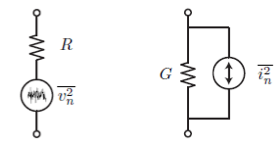
\includegraphics[scale=0.5]{pictures/widerstandrauschen}
	\columnbreak
	\begin{align*}
		S_{noise}(R) &=4kTR\\
		E_{noise}(R) &=\sqrt{4kTR}\\
		\overline{\nu^2_{n}} &=4kTRB\\
		\overline{i^2_{n}} &=4kTGB\\
		\nu_{rms} &= \sqrt{\overline{\nu^2_{n}}} = \sqrt{4kTRB}
	\end{align*}
	\begin{tabular}{ll}
		B:&Bandbreite\\
		T:&Temperatur in Kelvin(293K)\\
		k:&$1.38 \cdot 10^{-23}JK^{-1}$\\
		$S_{noise}(R)$:&Spektrale Dichte (Leistung)\\
		$E_{noise}(R)$:&Spannungsdichte\\
		$\nu_{RMS}$: & Rauschspannung\\
	\end{tabular}
\end{multicols}

\subsubsection{Widerstände in Serie}
\begin{minipage}{0.4\textwidth}
	\begin{center}
		\begin{circuitikz}[european, scale=2]
	\draw (0,0) to [R=$R1$, *-] (1,0) to [R=$R2$, -*] (2,0);
\end{circuitikz}
	\end{center}
\end{minipage}
\begin{minipage}{0.6\textwidth}
	\begin{align*}
		\overline{\nu^2_{n}}&=4kT(R1+R2)B=\overline{\nu^2_{n1}}+\overline{\nu^2_{n2}}\\
		\overline{i^2_{n}}&=4kT(G1+G2)B=\overline{i^2_{n1}}+\overline{i^2_{n2}}
	\end{align*}
\end{minipage}

\subsubsection{Spannungsteiler}
\begin{minipage}{0.4\textwidth}
	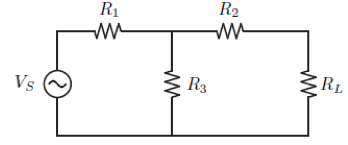
\includegraphics[scale=0.5]{pictures/seriewiderstand1}\\
	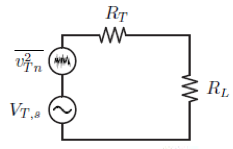
\includegraphics[scale=0.5]{pictures/seriewiderstand2}
\end{minipage}
\begin{minipage}{0.6\textwidth}
	Quellenumwandlung machen und dann Rauschen über Ersatzwiderstand ($R_T$) bestimmen.
	\begin{align*}
		V_{T,s}&=V_{s}\frac{R_{3}}{R_{1}+R_{3}}\\
		\overline{\nu^2_{Tn}}&=4kTR_{T}B=4kT(R_{2}+R_{1}\parallel R_{3})B
	\end{align*}
\end{minipage}

\subsection{Rauschen von RC-Netzwerken}
\begin{itemize}
  \item Kapazitäten (und Induktivitäten) rauschen nicht!
  \item Kapazitäten (und Induktivitäten) ändern die Bandbreite des Systems, d.h.
  beeinflussen dadurch die Rauschspannung
\end{itemize}
\begin{minipage}{9cm}
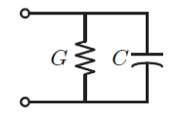
\includegraphics[scale=0.4]{pictures/rcnetzwerk}
\end{minipage}
\begin{minipage}{9cm}
\begin{gather*}
Z=\frac{1}{Y}=\frac{1}{G+j\omega C}=\frac{G-j\omega C}{G^2+\omega^2C^2}\\
\overline{\nu^2_{n}}=\frac{4kT}{2\pi}\int^{\infty}_{0}\frac{G}{G^2+\omega^2C^2}d\omega=\frac{kT}{C}\\
\overline{\nu_{n}}=\sqrt{\frac{kT}{C}}
\end{gather*}
\end{minipage}

\subsection{Rausch-Bandbreite}
\begin{multicols}{2}
	\begin{itemize}
  		\item Nicht 3dB-Bandbreite sondern das gesamte integrierte Rauschen wird
  			berechnet
  		\item $e_{on}$ Rauschspannung am Ausgang der Schaltung
  		\item $e_{in}$ Rauschspannung am Eingang der Schaltung
  		\item für höhere Filterodnung\\
  			\begin{tabular}{|l|l|}
  				\hline
  				Filter order&ENB\\\hline
  				1&$1.57 \cdot f_{c}$\\\hline
  				2&$1.11 \cdot f_{c}$\\\hline
  				3&$1.05 \cdot f_{c}$\\\hline
  				4&$1.025 \cdot f_{c}$\\\hline
  			\end{tabular}\\
  			ENB: Effective Noise Bandwidth
	\end{itemize}
	
	\columnbreak
	
	\begin{align*}
		e_{on} &= \sqrt{\int^{\infty}_{0}|A_{n(f)}|^2e^2_{in}df}
		\intertext{\textbf{für System 1. Ordnung:}}
		e_{on} &= e_{in}\sqrt{ \frac{1}{2 \pi RC} \frac{ \pi}{2}}
\end{align*}	
\end{multicols}

\subsection{Noise von Opamps}
\begin{multicols}{2}
	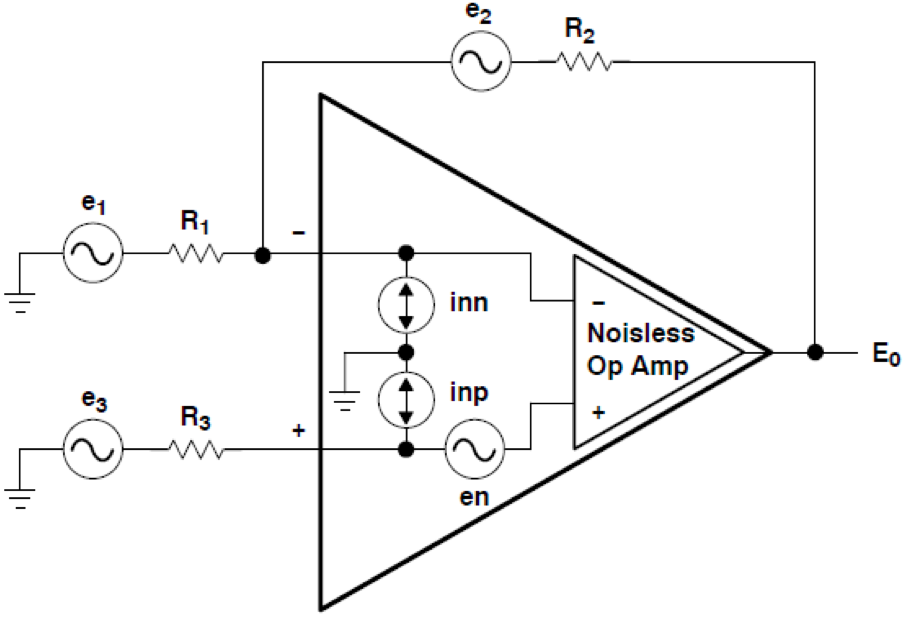
\includegraphics[scale=0.4]{pictures/oampnoise}
	\columnbreak
	
	\textbf{für CMOS-Opamps:} \\
	$R_3=0$ \\
	Gain A = $\frac{R1+R2}{R1}$ \\
	$e_{w}$:$\dfrac{Noise}{\sqrt{Hz}}$ (Aus Datenblatt) \\
	$f_{enc}$: noise corner frequenzcy (aus Datenblatt) \\
	ENB: Effective Noise Bandwidth \\
	$E_{Trms}=\sqrt{ENB \cdot 4kTR_{2}A+e_{w}^2A^2(f_{enc}\ln{\frac{f_{H}}{f_{L}}}+ENB)}$
\end{multicols}

\textbf{Gesamtfomel (Opamp und Widerstände)}\\
\begin{gather*}
E_{Trms}=\notag\\\sqrt{\int
\{4kTR_{2}(\frac{R_{1}+R_{2}}{R_{1}})+4kTR_{3}(\frac{R_{1}+R_{2}}{R_{1}})^2+((I_{nn})R_{2})^2+((I_{nn})R_{3}(\frac{R_{1}+R_{2}}{R_{1}}))^2+(e_{n}(\frac{R_{1}+R_{2}}{R_{1}}))^2\}df}
\end{gather*}


Vereinfacht 


Ist die Bandbreite $>>f_{enc}$ ( mind. 10x grösser) kann 1/f-Noise
vernachlässigt werden
\begin{itemize}
  \item Gain A=$\frac{R1+R2}{R1}$
  \item $e_{w}$: Noise/root(Hz)(Aus Datenblatt)
  \item ENB: Effective Noise Bandwidth ($1.51 \cdot GBW/A$)
\end{itemize}
\begin{gather*}
V_{noise}=\sqrt{4kT \cdot R_{2} \cdot A \cdot ENB+e_{w}^2 \cdot A^2 \cdot ENB}
\end{gather*}
